\section{Framework}
\label{sec:framework}

We present an open-source framework that translates natural-language strategic requirements into well-formed ATL/ATL$^\ast$ specifications. Figure~\ref{fig:tool_pipeline} shows the end-to-end pipeline. Requirements enter through a command-line or REST interface, or through the optionally patched \textsc{VITAMIN} model checker. At experiment time, the experiment orchestrator coordinates data access, model selection, optional fine-tuning, inference, and evaluation. For deployment, the \texttt{/generate} service resolves the requested model, dispatches local or API inference, and returns the generated formula with provenance metadata.

\subsection{Architecture}

The \emph{Dataset Manager} creates deterministic stratified splits and holds curated few-shot exemplars out of evaluation. Model configurations identify each local checkpoint or API deployment and its decoding settings. Open-weight models may first undergo LoRA fine-tuning; local or API inference then produces predictions and provenance, which exact-match and LLM evaluators convert into accuracy, agreement, and efficiency metrics.

\usetikzlibrary{arrows.meta, positioning, backgrounds, calc}
\begin{figure}[t]
\centering
\resizebox{0.95\columnwidth}{!}{%
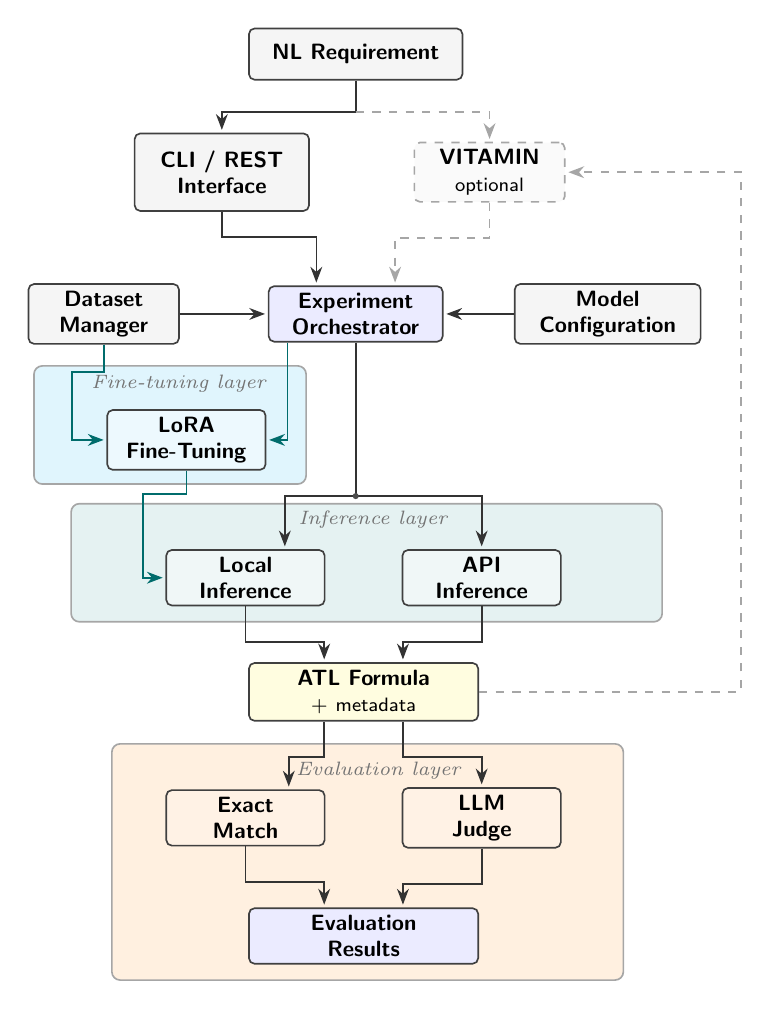
\begin{tikzpicture}[
    font=\footnotesize\sffamily,
    >=Stealth,
    box/.style={
        rectangle, draw=black!75, semithick, rounded corners=2pt,
        align=center, fill=white, minimum height=6.5mm,
        inner xsep=3pt, inner ysep=2.5pt
    },
    io/.style={box, fill=gray!8},
    core/.style={box, fill=blue!8},
    data/.style={box, fill=yellow!12},
    train/.style={box, fill=cyan!7},
    infer/.style={box, fill=teal!6},
    eval/.style={box, fill=orange!10},
    optionalbox/.style={box, fill=gray!4, draw=gray!70, dashed},
    layerbox/.style={
        rounded corners=3pt, draw=black!35, semithick, fill=#1
    },
    lbl/.style={font=\scriptsize, inner sep=1pt},
    arr/.style={->, semithick, draw=black!80, shorten >=1pt},
    trainarr/.style={->, semithick, draw=teal!85!black, shorten >=1pt},
    optional/.style={->, semithick, dashed, draw=gray!70, shorten >=1pt},
    line/.style={semithick, draw=black!80}
]

% Requirement and alternative entry points
\node[io, text width=2.5cm] (request) at (0, 6.8)
    {\textbf{NL Requirement}};
\node[io, text width=57pt, minimum height=28pt] (direct) at (-1.7, 5.3)
    {\textbf{CLI / REST}\\\textbf{Interface}};
\node[optionalbox, text width=1.7cm] (vit) at (1.7, 5.3)
    {\textbf{\textsc{VITAMIN}}\\{\scriptsize optional}};

% Control layer and experiment-time inputs
\node[io, text width=1.7cm] (dm) at (-3.2, 3.5)
    {\textbf{Dataset}\\\textbf{Manager}};
\node[core, text width=2.0cm] (control) at (0, 3.5)
    {\textbf{Experiment}\\\textbf{Orchestrator}};
\node[io, text width=2.15cm] (registry) at (3.2, 3.5)
    {\textbf{Model}\\\textbf{Configuration}};

% Fine-tuning occupies its own row above inference
\node[train, text width=1.8cm] (ft) at (-2.15, 1.9)
    {\textbf{LoRA}\\\textbf{Fine-Tuning}};
\node[infer, text width=1.8cm] (local) at (-1.4, 0.15)
    {\textbf{Local}\\\textbf{Inference}};
\node[infer, text width=1.8cm] (api) at (1.6, 0.15)
    {\textbf{API}\\\textbf{Inference}};

% Formula and evaluation outputs
\node[data, text width=2.7cm] (formula) at (0.1, -1.3)
    {\textbf{ATL Formula}\\{\scriptsize $+$ metadata}};
\node[eval, text width=1.8cm] (em) at (-1.4, -2.9)
    {\textbf{Exact}\\\textbf{Match}};
\node[eval, text width=1.8cm] (judge) at (1.6, -2.9)
    {\textbf{LLM}\\\textbf{Judge}};
\node[core, text width=2.7cm] (metrics) at (0.1, -4.4)
    {\textbf{Evaluation}\\\textbf{Results}};

% Freeform layer paths: edit the corner coordinates independently.
\begin{scope}[on background layer, xshift=21pt, xscale=1.44]
\path[layerbox=cyan!12] (-3.35, 1.34) rectangle (-0.95, 2.84);
\end{scope}
\begin{scope}[on background layer, xshift=0pt, xscale=1.39]
\path[layerbox=teal!10] (-2.60, -0.41) rectangle (2.80, 1.09);
\end{scope}
\begin{scope}[on background layer, xshift=1pt, xscale=1.16]
\path[layerbox=orange!12] (-2.70, -4.96) rectangle (2.90, -1.96);
\end{scope}
% Free-standing labels: adjust these coordinates independently of the boxes.
\node[font=\scriptsize\itshape, text=black!55, anchor=north west]
    at (-3.48, 2.85) {Fine-tuning layer};
\node[font=\scriptsize\itshape, text=black!55, anchor=north west]
    at (-0.85, 1.12) {Inference layer};
\node[font=\scriptsize\itshape, text=black!55, anchor=north west]
    at (-0.88, -2.07) {Evaluation layer};

% A requirement either enters directly or through the optional client
\coordinate (entryfork) at ([yshift=-0.4cm]request.south);
\draw[line] (request.south) -- (entryfork);
\draw[arr] (entryfork) -| (direct.north);
\draw[optional] (entryfork) -| (vit.north);
\draw[arr] (direct.south) -- ++(0,-0.32)
    -| ([xshift=-0.5cm]control.north);
\draw[optional] (vit.south) -- ++(0,-0.45)
    -| ([xshift=0.5cm]control.north);

% Dataset and model configuration enter from opposite sides
\draw[arr] (dm.east) -- (control.west);
\draw[arr] (registry.west) -- (control.east);

% Optional training path
\draw[trainarr] (dm.south) -- ++(0,-0.35) -- ++(-0.40,0)
    |- (ft.west);
\draw[trainarr] ([xshift=0.25cm]control.south west) -- ++(0,-0.35)
    |- (ft.east);
\draw[trainarr] (ft.south) -- ++(0,-0.30) -- ++(-0.55,0)
    |- (local.west);

% Runtime dispatch reaches each inference backend from above
\coordinate (inferfork) at ([yshift=-1.95cm]control.south);
\draw[line] (control.south) -- (inferfork);
\draw[arr] (inferfork) -| ([xshift=0.5cm]local.north);
\draw[arr] (inferfork) -| (api.north);
\fill[black!70] (inferfork) circle (1.1pt);

% Both backends enter the formula box perpendicularly
\draw[arr] (local.south) -- ++(0,-0.45)
    -| ([xshift=-0.5cm]formula.north);
\draw[arr] (api.south) -- ++(0,-0.45)
    -| ([xshift=0.5cm]formula.north);

% The translated formula is returned to the optional client
\coordinate (vitreturn) at (registry.east |- vit.east);
\draw[optional] (formula.east) -| ([xshift=0.5cm]vitreturn)
    -- (vit.east);

% Experimental evaluation remains downstream of generation
\draw[arr] ([xshift=-0.5cm]formula.south) -- ++(0,-0.45)
    -| ([xshift=0.55cm]em.north);
\draw[arr] ([xshift=0.5cm]formula.south) -- ++(0,-0.45)
    -| (judge.north);
\draw[arr] (em.south) -- ++(0,-0.45)
    -| ([xshift=-0.5cm]metrics.north);
\draw[arr] (judge.south) -- ++(0,-0.45)
    -| ([xshift=0.5cm]metrics.north);

\end{tikzpicture}%
}
\caption{Framework overview. Black arrows show translation and evaluation; teal arrows show optional open-weight fine-tuning. Dashed gray arrows show the optional \textsc{VITAMIN} path, which sends a requirement to the translation service and receives the generated formula.}
\label{fig:tool_pipeline}
\end{figure}

\paragraph{Prompting and Output Parsing.}
\label{subsec:prompting}
The fixed system prompt specifies the ATL/ATL$^\ast$ syntax, scope conventions, and the treatment of targeted ambiguities. It requires all admissible readings for multi-reading requirements. Few-shot exemplars are held out of every split, and output parsing canonicalizes incidental surface differences before scoring; exact match still requires the complete set of gold formulas. For full prompt and exemplars see the appendix.

\paragraph{Deployment, Privacy, and Reproducibility.}
\label{subsec:scale}
Local open-weight checkpoints are LoRA fine-tuned~\cite{hu2022lora}, using $4$-bit QLoRA~\cite{dettmers2023qlora} for larger models, so privacy-sensitive requirements can remain on premises; the same interface also supports Azure OpenAI endpoints. The orchestrator decouples split and training seeds, uses one canonical stratified split for the reported results, and supports shared-fold cross-validation for future estimates of split-induced variance.

\subsection{Model-Checker Integration}
\label{subsec:integration}
We integrate the framework with \textsc{VITAMIN}, an established strategic-logic model checker~\cite{DBLP:conf/ifaamas/0001M25}. Translation runs as a FastAPI service, and a thin client routes ATL requests to it before falling back to the checker's native generation if necessary. The verifier's own parser accepts only well-formed translated formulas; the interface and screenshot are provided in the appendix.